\documentclass[aspectratio=169]{beamer}
%
% Choose how your presentation looks.
%
% For more themes, color themes and font themes, see:
% http://deic.uab.es/~iblanes/beamer_gallery/index_by_theme.html
%
\mode<presentation>
{
  \usetheme{metropolis}      % or try Darmstadt, Madrid, Warsaw, ...
  \usecolortheme{default} % or try albatross, beaver, crane, ...
  \usefonttheme{structurebold}  % or try serif, structurebold, ...
  \setbeamercolor{background canvas}{bg=white}
  \setbeamertemplate{navigation symbols}{}
  \setbeamertemplate{bibliography item}{\insertbiblabel}
  %\setbeamertemplate{caption}[numbered]
} 
\usepackage[english]{babel}
\usepackage[utf8x]{inputenc}
\usepackage{listings}             % Include the listings-package
\usepackage{bm}	% math package

\hypersetup{
    colorlinks = true,
    linkcolor = {black},
    urlcolor = {blue}
}

\DeclareMathOperator*{\argmin}{arg\,min}

\title[Deep Learning and Temporal Data Processing]{Deep Learning and Temporal Data Processing}
\subtitle{3 - Recurrent Neural Networks}
\institute{University of Modena and Reggio Emilia}
\author{Andrea Palazzi}
\date{June 21th, 2017}

\def\thisframelogos{}

\newcommand{\framelogo}[1]{\def\thisframelogos{#1}}

\addtobeamertemplate{frametitle}{}{%
\begin{tikzpicture}[remember picture,overlay]
\node[anchor=north east] at (current page.north east) {%
    \foreach \img in \thisframelogos {%
        %\hspace{.5ex}%
        \includegraphics[height=3.5ex]{\img}%
    }%
};
\end{tikzpicture}}

\begin{document}

\framelogo{logo_unimore_white.png}

\bgroup
\renewcommand{\insertframenumber}{}
\begin{frame}[noframenumbering]
  \titlepage
\end{frame}
\egroup
\begin{frame}{Agenda}
  \tableofcontents
\end{frame}


%%%%%%%%%%%%%%%%%%%%%%%%%%%%%%%%%%%%%%%%%%%%%%%%%%%%%%%%%%%%%%%%%%
%%%%%%%%%%%%%%%%%%%%%%%%%%%%%%%%%%%%%%%%%%%%%%%%%%%%%%%%%%%%%%%%%%
%%%%%%%%%%%%%%%%%%%%%%%%%%%%%%%%%%%%%%%%%%%%%%%%%%%%%%%%%%%%%%%%%%

\section{Introduction}

%%%%%%%%%%%%%%%%%%%%%%%%%%%%%%%%%%%%%%%%%%%%%%%%%%%%%%%%%%%%%%%%%%

\begin{frame}{Recurrent Neural Networks}
test \cite{cybenko1989approximation}
\end{frame}

%%%%%%%%%%%%%%%%%%%%%%%%%%%%%%%%%%%%%%%%%%%%%%%%%%%%%%%%%%%%%%%%%%

\begin{frame}{Recurrent Neural Networks}
In \textbf{feedforward neural network} computation flows directly from input $\bm{x}$ through intermediate layers $\bm{h}$ to output $\bm{y}$.\\
\vspace{0.5cm}
Conversely, some networks topology feature feedback connections, in other words model outputs are fed back into the model itself.\\
\vspace{0.5cm}
The term \textbf{recurrent neural networks} defines this family of models.

\end{frame}

%%%%%%%%%%%%%%%%%%%%%%%%%%%%%%%%%%%%%%%%%%%%%%%%%%%%%%%%%%%%%%%%%%

\begin{frame}{Recurrent Neural Networks}
Recurrent neural networks (RNN) are \textbf{specialized for processing sequences}. Similarly, we saw that convolutional neural networks feature specialized architecture for processing images.\\
\vspace{0.4cm}
RNNs boast a \textbf{much wider API with respect to feedforward neural networks}. Indeed, these models can deal with \textit{sequences} in the input, in the output or even both.
\begin{figure}
\begin{tabular}{c}
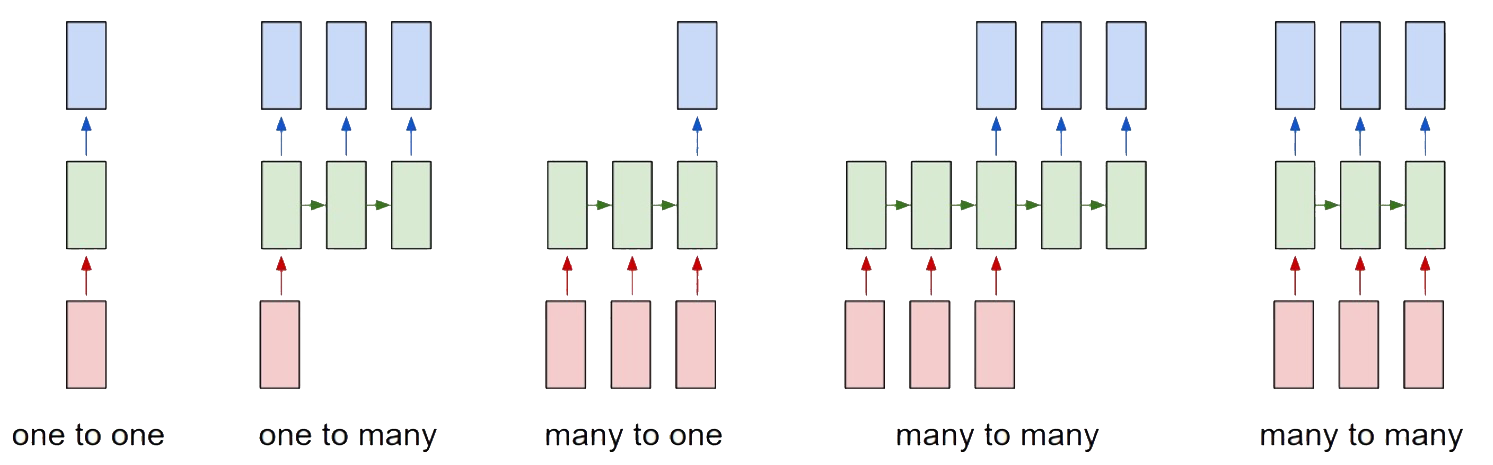
\includegraphics[width=0.8\textwidth]{img/rnn/rnn_api.png}
\end{tabular}
\end{figure}
\end{frame}

%%%%%%%%%%%%%%%%%%%%%%%%%%%%%%%%%%%%%%%%%%%%%%%%%%%%%%%%%%%%%%%%%%

\begin{frame}{Vanilla RNN}
\begin{columns}
\begin{column}{0.3\textwidth}
\begin{tabular}{c}
	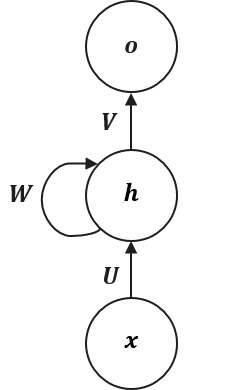
\includegraphics[width=0.7\textwidth]{img/rnn/vanilla_rnn.png}
\end{tabular}
\end{column}
\begin{column}{0.7\textwidth}
The vanilla RNN is provided with three sets of parameters:
\begin{itemize}
	\item $\bm{U}$ maps inputs to the hidden state
	\item $\bm{W}$ parametrizes hidden state transition
	\item $\bm{V}$ maps hidden state to output 
\end{itemize}
\vspace{0.5cm}
System dynamics is as simple as:
\begin{equation}
	\begin{cases}
	\bm{h}^{(t)} = \phi(\bm{W}\,\bm{h}^{(t-1)} + \bm{U}\,\bm{x}^{(t)})\\
	\bm{o}^{(t)} = \bm{V}\,\bm{h}^{(t)}
	\end{cases}
\end{equation}
\end{column}
\end{columns}
\end{frame}

%%%%%%%%%%%%%%%%%%%%%%%%%%%%%%%%%%%%%%%%%%%%%%%%%%%%%%%%%%%%%%%%%%

\begin{frame}{Intuition about Hidden State}
\begin{columns}
\begin{column}{0.3\textwidth}
\begin{tabular}{c}
	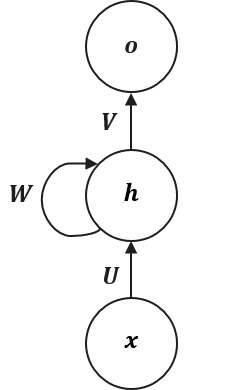
\includegraphics[width=0.7\textwidth]{img/rnn/vanilla_rnn.png}
\end{tabular}
\end{column}
\begin{column}{0.7\textwidth}
The hidden state $\bm{h}^{(t)}$ can be intuitively viewed as a \textit{lossy} summary of the sequence of past inputs fed to the network, in which are stored the main task-relevant aspects of the past sequence of inputs up to time $t$.\\
\vspace{0.5cm}
Since the an input sequence of arbitrary length $(\bm{x}^{(1)}, \bm{x}^{(2)}, ..., \bm{x}^{(t)})$ is mapped into a fixed size vector $\bm{h}^{(t)}$, this summary is necessarily lossy.
\end{column}
\end{columns}
\end{frame}

%%%%%%%%%%%%%%%%%%%%%%%%%%%%%%%%%%%%%%%%%%%%%%%%%%%%%%%%%%%%%%%%%%

\begin{frame}{Unfolding the Computational Graph}
A recurrent computational graph can be unfolded into a sequential computational graph with a repetitive structure.
\begin{equation*}
\bm{h}^{(t)} = f(\bm{h}^{t-1}, \bm{x}^{(t)}; \bm{\theta})
\end{equation*}
\begin{figure}
\begin{tabular}{c}
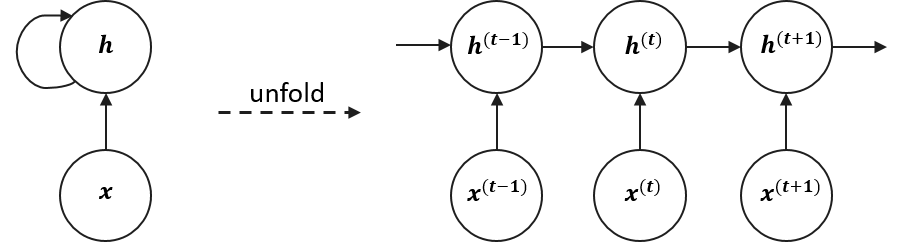
\includegraphics[width=0.8\textwidth]{img/rnn/rnn_unfold.png}
\end{tabular}
\end{figure}
\begin{columns}
\end{columns}
\end{frame}

%%%%%%%%%%%%%%%%%%%%%%%%%%%%%%%%%%%%%%%%%%%%%%%%%%%%%%%%%%%%%%%%%%

\begin{frame}{Backpropagation Through Time}
how to unroll a recursive graph
\end{frame}

%%%%%%%%%%%%%%%%%%%%%%%%%%%%%%%%%%%%%%%%%%%%%%%%%%%%%%%%%%%%%%%%%%

\begin{frame}{The Challenge of Long-Term Dependencies}
Vanishing and exploding gradient problem.
\end{frame}

%%%%%%%%%%%%%%%%%%%%%%%%%%%%%%%%%%%%%%%%%%%%%%%%%%%%%%%%%%%%%%%%%%

\begin{frame}{Long Short-Term Memory networks}
Vanishing and exploding gradient problem.
\end{frame}

%%%%%%%%%%%%%%%%%%%%%%%%%%%%%%%%%%%%%%%%%%%%%%%%%%%%%%%%%%%%%%%%%%

\begin{frame}{Notes}
No matter how's the network topology, during backpropagation the network is unfolded in a DAG, so there are no loops.
\end{frame}

%%%%%%%%%%%%%%%%%%%%%%%%%%%%%%%%%%%%%%%%%%%%%%%%%%%%%%%%%%%%%%%%%%
%%%%%%%%%%%%%%%%%%%%%%%%%%%%%%%%%%%%%%%%%%%%%%%%%%%%%%%%%%%%%%%%%%
%%%%%%%%%%%%%%%%%%%%%%%%%%%%%%%%%%%%%%%%%%%%%%%%%%%%%%%%%%%%%%%%%%

\section{Credits}
\begin{frame}{Credits}
These slides heavily borrow from the following Stanford course:
\begin{itemize}
\item \url{http://cs231n.stanford.edu/}
\end{itemize}
if you want to deepen your knowledge of these concepts, I'd really suggest to start from here!\\
\vspace{0.2cm}
Also, nice convolution animations are taken from here:
\begin{itemize}
\item \url{https://github.com/vdumoulin/conv_arithmetic}
\end{itemize}
\end{frame}

%%%%%%%%%%%%%%%%%%%%%%%%%%%%%%%%%%%%%%%%%%%%%%%%%%%%%%%%%%%%%%%%%%
%%%%%%%%%%%%%%%%%%%%%%%%%%%%%%%%%%%%%%%%%%%%%%%%%%%%%%%%%%%%%%%%%%
%%%%%%%%%%%%%%%%%%%%%%%%%%%%%%%%%%%%%%%%%%%%%%%%%%%%%%%%%%%%%%%%%%

\begin{frame}[t, allowframebreaks]
\frametitle{References}
\bibliographystyle{abbrv}
\bibliography{bibliography}
\end{frame}
\end{document}